%scrrprt ist eine Klasse für Berichte und längere Arbeiten
\documentclass[11pt,a4paper]{scrreprt}
%ermöglicht die Eingabe von Umlauten usw. ohne Codierung
\usepackage[utf8]{inputenc}
%Schriften werden mit einer passenden Kodierung für europäische Zeichen ausgegeben
\usepackage[T1]{fontenc}
%Passt Dokumentelemente an die Konventionen der deutschen Sprache (neue Rechtschreibung) an, z.b. Datumsangaben, Silbentrennung
\usepackage[ngerman]{babel}
%Grafikpaket
\usepackage{graphicx}
\usepackage{scrpage2}
\usepackage{hyperref}
\pagestyle{scrheadings}
\clearscrheadfoot
%\Chapter sorgt dafür, dass kein Seitenvorschub auftritt.
\makeatletter
\newcommand\Chapter{%
                    \par\vspace{0.01cm}% anpassen
                    \global\@topnum\z@
                    \@afterindentfalse
                    \secdef\@chapter\@schapter}
\makeatother


\begin{document}
\begin{titlepage}
	\centering
	{\scshape\LARGE Universität Leipzig \par}
	\vspace{1cm}
	{\scshape\Large Information Retrieval Laborprojekt \par}
	\vspace{2cm}
	{\huge\bfseries Evaluation der Geocache-Suchmaschine \par}
	\vspace{2cm}
	{\Large\itshape Steven Lehmann, Fabian Ziegner, Christian Schlecht \par}
	\vfill
	supervised by \par
	Jun.-Prof. Dr.~Martin \textsc{Potthast}
	\vfill
	{\large \today \par}
\end{titlepage}
\tableofcontents

\ihead{11.12.2017}
\ohead{Gruppe Geocache-Search}
\cfoot{\pagemark}

\Chapter{Begriffserklärungen}
\section{Geocaching}
Unter Geocaching wird eine Art Schnitzeljagd verstanden. Das Wort leitet sich vom lateinischen $\gamma$$\widetilde{\eta}$, gē, stehend für ``Erde`` und dem englischen ``cache`` für ``geheimes Lager`` ab. Ziel ist es, mit Hilfe von GPS-Koordinaten und/oder veröffentlichen Tipps einen versteckten Behälter - den sogenannten ``Geocache`` (auch kurz ``Cache``)  - zu finden. In der Regel beinhaltet dieser Behälter ein Logbuch, in welches sich die Geocacher bei erfolgreicher Suche eintragen können. Zusätzlich, sofern es die Größe des Behälters hergibt, sind oftmals kleine Gegenständen zum Tausch vorhanden. Wichtig ist es, während der gesamten Zeit möglichst unentdeckt zu bleiben, sodass der Cache stets verborgen bleibt. Nach Beendigung der Suche wird der Cache wieder an seine ursprüngliche Position gebracht.

Es gibt eine ganze Reihe Arten von Geocaches. Vom einfachen traditionelle Caches, über Multi-Caches und Rätsel-Caches bis hin zu virtuellen Caches können Suchen veranstaltet werden.

Fairness wird beim Geocaching groß geschrieben. Personen, die den Cache veröndern, mutmaßlich zerstören, entfernen oder Dinge daraus stehlen wird größter Missmut entgegengestellt.

\Chapter{Motivation}
\section{Domäne}
\subsection{Geocaching als Sport}
Geocaching erfreut sich zunehmender Beliebtheit unter der Bevölkerung, obwohl es in gewissem Sinne das Ziel ist, geheim zu agieren. Dieser Sport kann von Menschen aller Altersgruppen und körperlicher Verfassung betrieben werden, da in praktisch jeder Region (Wald, Stadt, Parkanlagen, Gebirge, \dots) Caches versteckt und gefunden werden können. Unterbewusst wird dadurch die Gesundheit gefördert. Aus dieser Hinsicht ist der Sport in jedem Fall zu unterstützen. 

\subsection{technischer Stand}
Mittlerweile wird Geocaching durch das Internet stark unterstützt und vereinfacht. Während in den Anfängen (1980er Jahre) die Hinweise und Koordinaten meist verbal oder handschriftlich verbreitet wurden, gibt es heutzutage diverse Plattformen und Foren, um sich auszutauschen. Zu den bekanntesten gehören hier \href{geocaching.com}{geocaching.com} und \href{opencaching.de}{opencaching.de} im deutschsprachigen Raum. Diese Seiten agieren im Wesentlichen als Foren zum Austausch mit anderen Cachern. Sie bieten zwar die Möglichkeit der Suche, jedoch wird hierbei auf eine Datenbank zurückgegriffen, aus welcher mittels SQL-Anweisungen Suchanfragen bearbeitet werden. Wir haben keinen Anbieter feststellen können, der bei der Suche Methoden des Information Retrieval, d.h. Verwendung eines Index und Retrieval-Modells, anwendet. An dieser Stelle wird im Rahmen dieses Projekts prototypisch gearbeitet. 

\section{Dokumentkorpus}
Die Geocaching Suchmaschine soll für Geocaches in Deutschland angewendet werden. Aus diesem Grund wurde als Dokumentkorpus eine Sammlung von allen \footnote{Stand 24.04.18} Geocaches in Deutschland, welche auf \href{opencaching.de}{opencaching.de} veröffentlicht sind, gewählt. Der Korpus beläuft sich damit auf eine Größe von ca. 20.000 Caches. Aufgrund des Mehraufwandes eines Web-Crawls wurden diese manuell heruntergeladen. Die Dokumentsammlung kann also als statisch betrachtet werden. 

\subsection{Dokumentstruktur}
Jedes Dokument kann von opencaching.de in diversen verschiedenen Formaten heruntergeladen werden, darunter auch direkt von GPS-System verwertbare Formate. Aufgrund der Vollständigkeit der Information wurden in diesem Rahmen Caches im .txt-Format verwendet. 

Das Dokument wird bereits beim Herunterladen in eine wohlgeformte Struktur gebracht. Die Abbildung \ref{img:struktur} zeigt einen Ausschnitt. Es lässt sich eine Art Key-Value-Struktur erkennen, welche das spätere Parsing der Dokumente vereinfacht, sodass eine maximale Korrektheit gewährleistet werden kann.
Interessant ist hierbei, dass durch dieses Dokument sämtliche Informationen aus der Web-Darstellung übernommen werden, die Informationen sind also a prior vollständig.

\begin{figure}
	\centering
	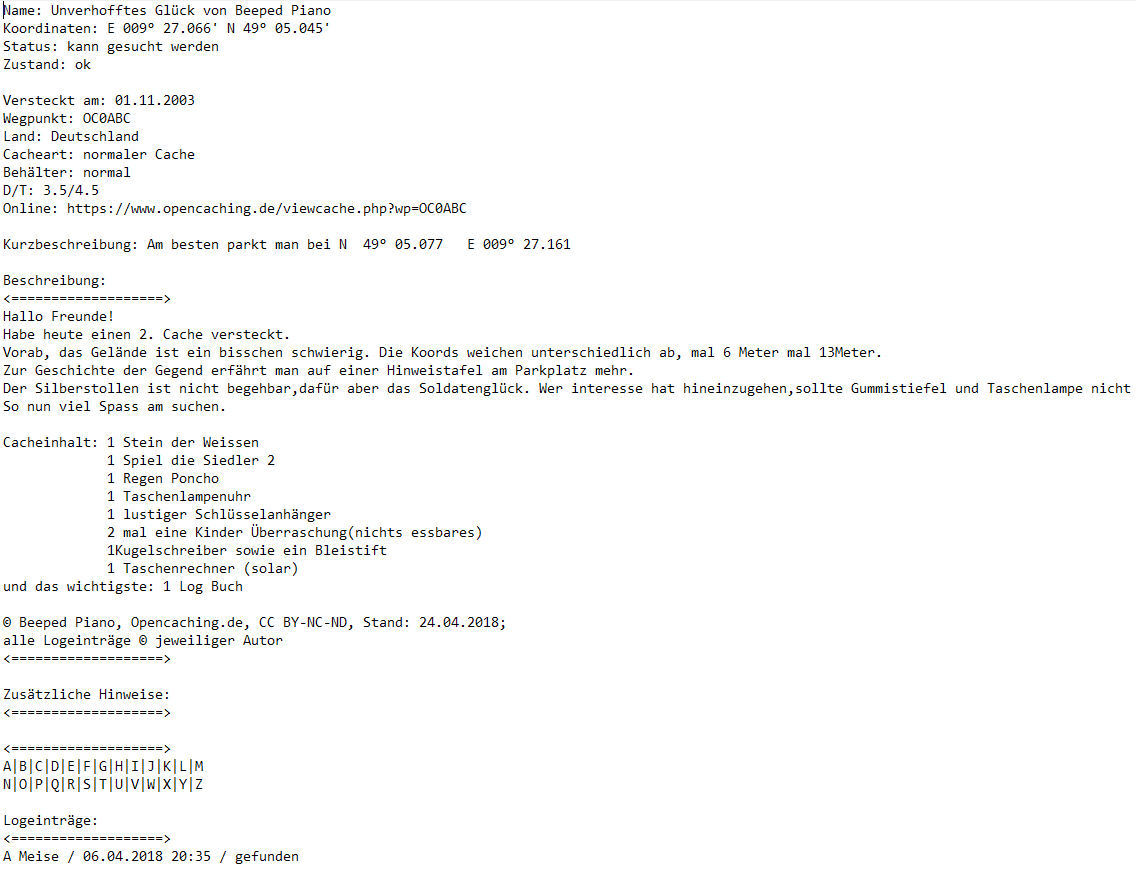
\includegraphics[height=0.6\textheight]{cache_struktur.png}
	\caption{Dokumenstruktur eines Geocaches}
	\label{img:struktur}
\end{figure}


\Chapter{Architektur}
tbc


\Chapter{Evaluation}
tbc
\end{document}